%%%%%%%%%%%%%%%%%%%%%%%%%%%%%%%%%%%%%%%%%%%%%%%%%%%%%%%%%%%%%%%%%%%%%%%%%%%%%%%%%%%%
% Do not alter this block (unless you're familiar with LaTeX
\documentclass{article}
\usepackage[margin=1in]{geometry} 
\usepackage{amsmath, amsthm, amssymb,amsfonts, fancyhdr, color, comment, graphicx, environ}
\usepackage{xcolor}
\usepackage{mdframed}
\usepackage[shortlabels]{enumitem}
\usepackage{indentfirst}
\usepackage{hyperref}
\usepackage{algorithm2e}
\usepackage{graphicx}
\usepackage{wrapfig}
\usepackage{hyperref}
\usepackage{listings}
\lstset{ 
  language=R,                     % the language of the code
  basicstyle=\normalsize\ttfamily, % the size of the fonts that are used for the code
  numbers=left,                   % where to put the line-numbers
  numberstyle=\normalsize\color{gray},  % the style that is used for the line-numbers
  stepnumber=1,                   % the step between two line-numbers. If it is 1, each line
                                  % will be numbered
  numbersep=5pt,                  % how far the line-numbers are from the code
  backgroundcolor=\color{white},  % choose the background color. You must add \usepackage{color}
  showspaces=false,               % show spaces adding particular underscores
  showstringspaces=false,         % underline spaces within strings
  showtabs=false,                 % show tabs within strings adding particular underscores
  frame=single,                   % adds a frame around the code
  rulecolor=\color{black},        % if not set, the frame-color may be changed on line-breaks within not-black text (e.g. commens (green here))
  tabsize=2,                      % sets default tabsize to 2 spaces
  captionpos=b,                   % sets the caption-position to bottom
  breaklines=true,                % sets automatic line breaking
  breakatwhitespace=false,        % sets if automatic breaks should only happen at whitespace
  keywordstyle=\color{black},      % keyword style
  commentstyle=\color{gray},   % comment style
  stringstyle=\color{teal}      % string literal style
} 
\hypersetup{
    colorlinks=true,
    linkcolor=blue,
    filecolor=magenta,      
    urlcolor=blue,
}


\pagestyle{fancy}


\newenvironment{problem}[2][Problem]
    { \begin{mdframed}[backgroundcolor=gray!20] \textbf{#1 #2} \\}
    {  \end{mdframed}}

% Define solution environment
\newenvironment{solution}
    {\textit{Solution:}}
    {}

\renewcommand{\qed}{\quad\qedsymbol}

% prevent line break in inline mode
\binoppenalty=\maxdimen
\relpenalty=\maxdimen

%%%%%%%%%%%%%%%%%%%%%%%%%%%%%%%%%%%%%%%%%%%%%
%Fill in the appropriate information below
\lhead{Pengju Zhang}
\rhead{CSC-424} 
\chead{\textbf{Assignment 2}}
%%%%%%%%%%%%%%%%%%%%%%%%%%%%%%%%%%%%%%%%%%%%%

\begin{document}
%problem 1
\begin{problem}{1}
\textbf{[20 pts]}
Perform, by hand, the following calculations from linear algebra. For the following matrices and vectors. Submit a copy of your answers either in a high-quality scan or photo (unreadable or clipped answers will not receive credit) or you may format it carefully in Word with equation editor showing all work. Note that Z has changed from last week, so re-do a) and b) here. Note: these numbers are different from homework 1!
\begin{equation}
Z = 
\begin{bmatrix}
1 & 2 \\
1 & -3 \\
1 & 4 \\
1 & -1
\end{bmatrix}, 
Y = 
\begin{bmatrix}
0 \\
1 \\
4 \\
-3
\end{bmatrix}
\end{equation}
\end{problem}
\begin{solution}
	\begin{figure}[h]
		\centering
		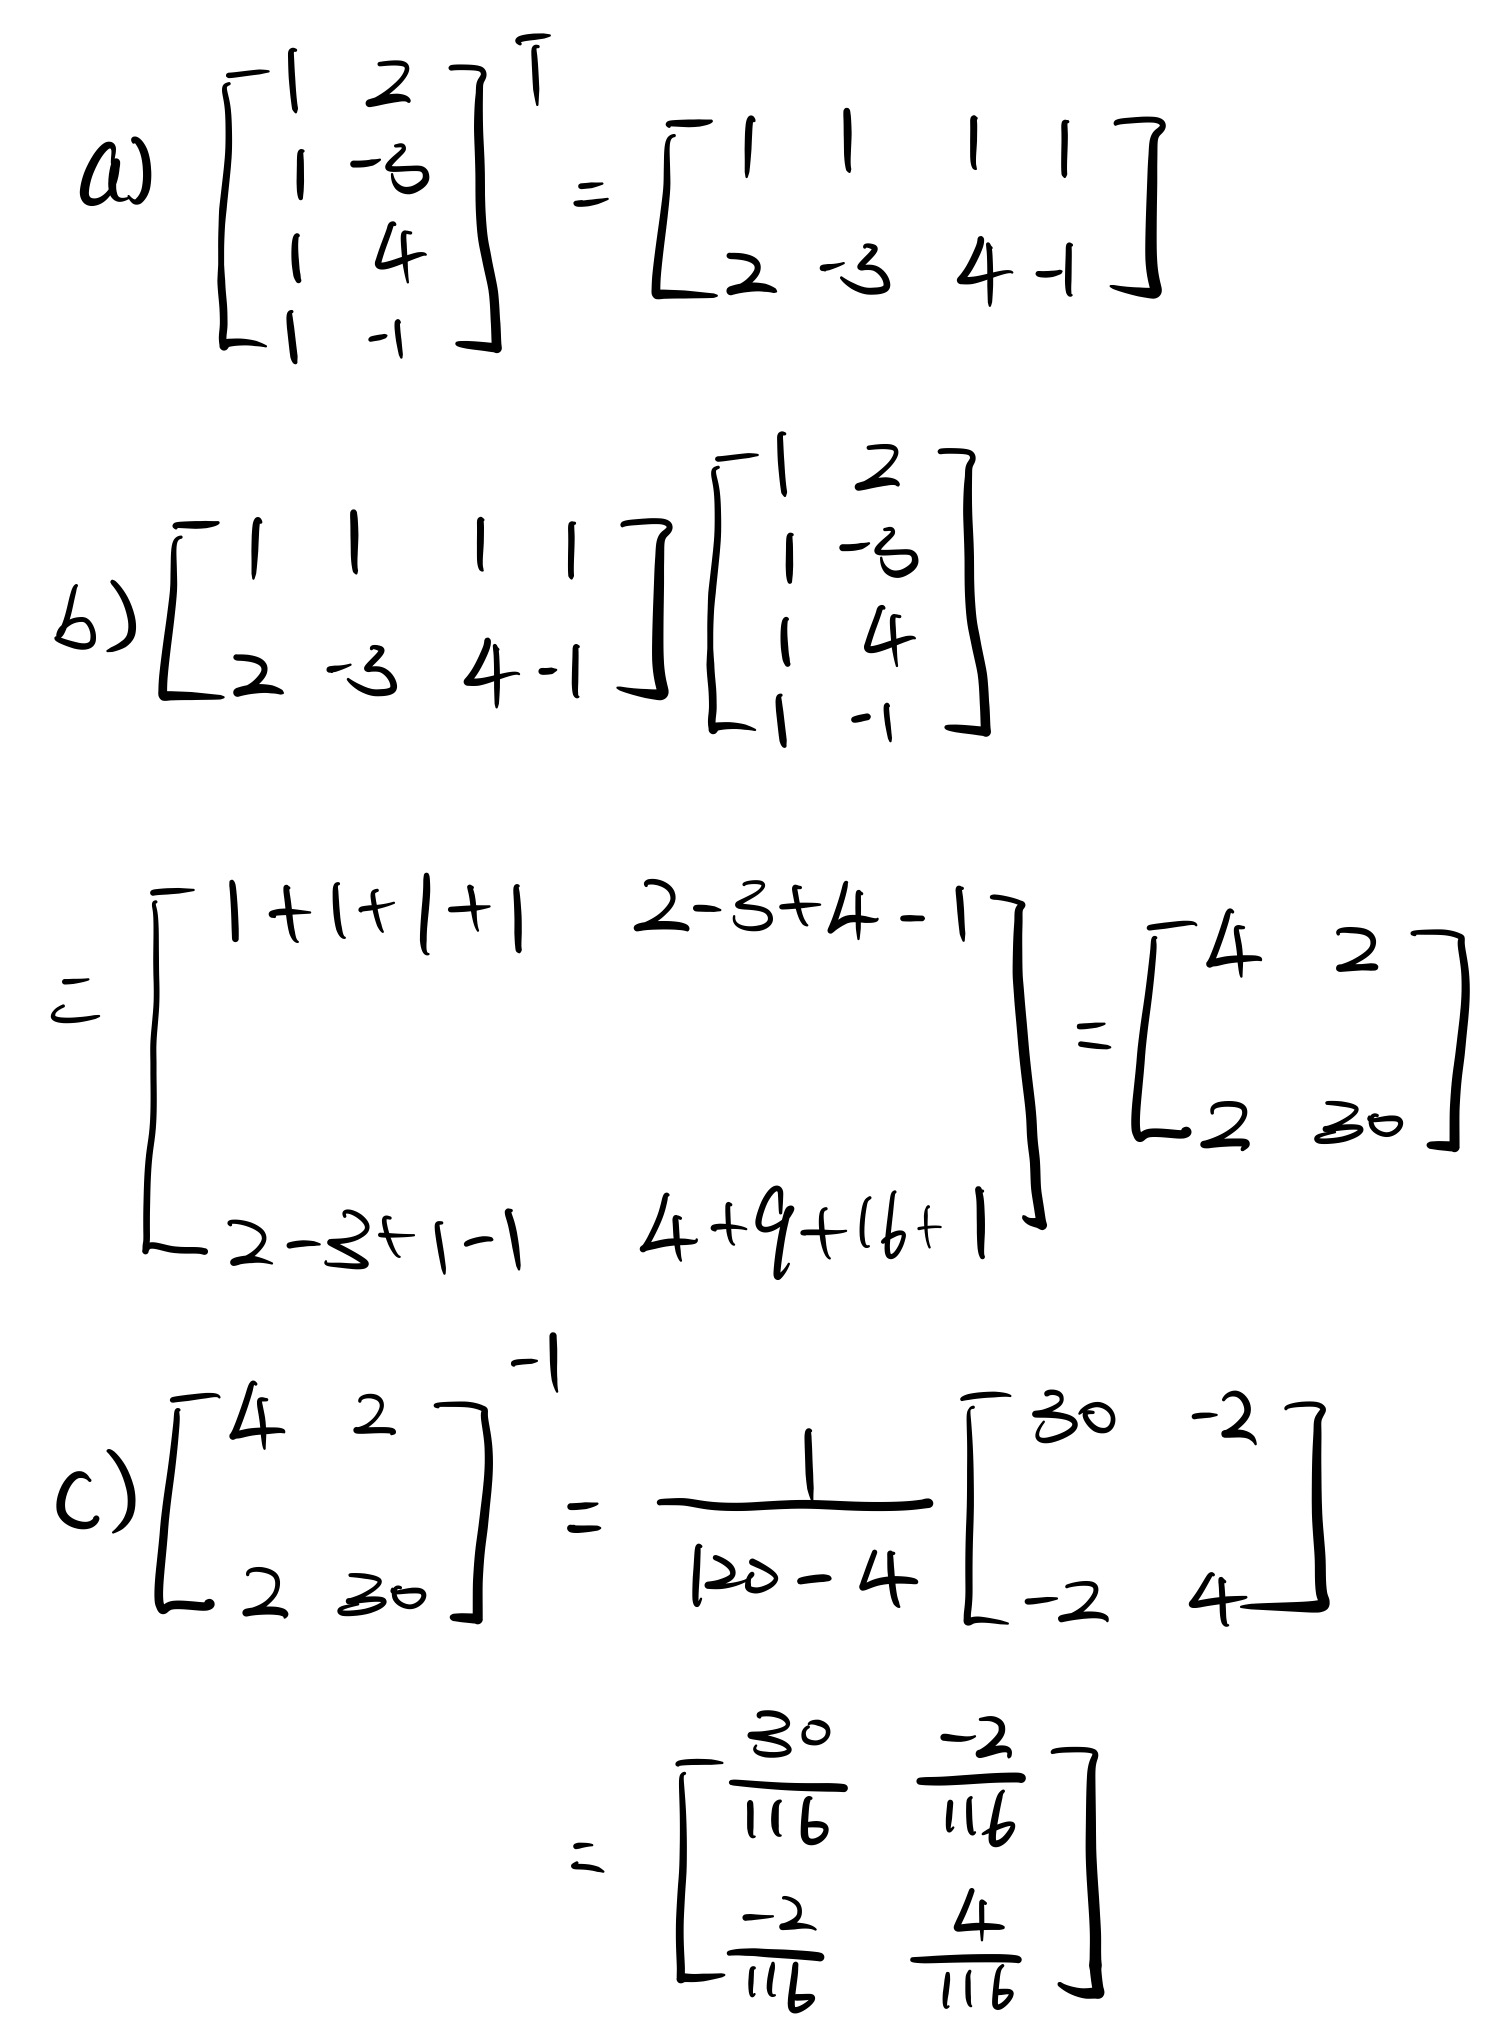
\includegraphics[width=0.7\textwidth]{figure1_Rplot.jpg}
	\end{figure}
\newpage
	\begin{figure}[h]
		\centering
		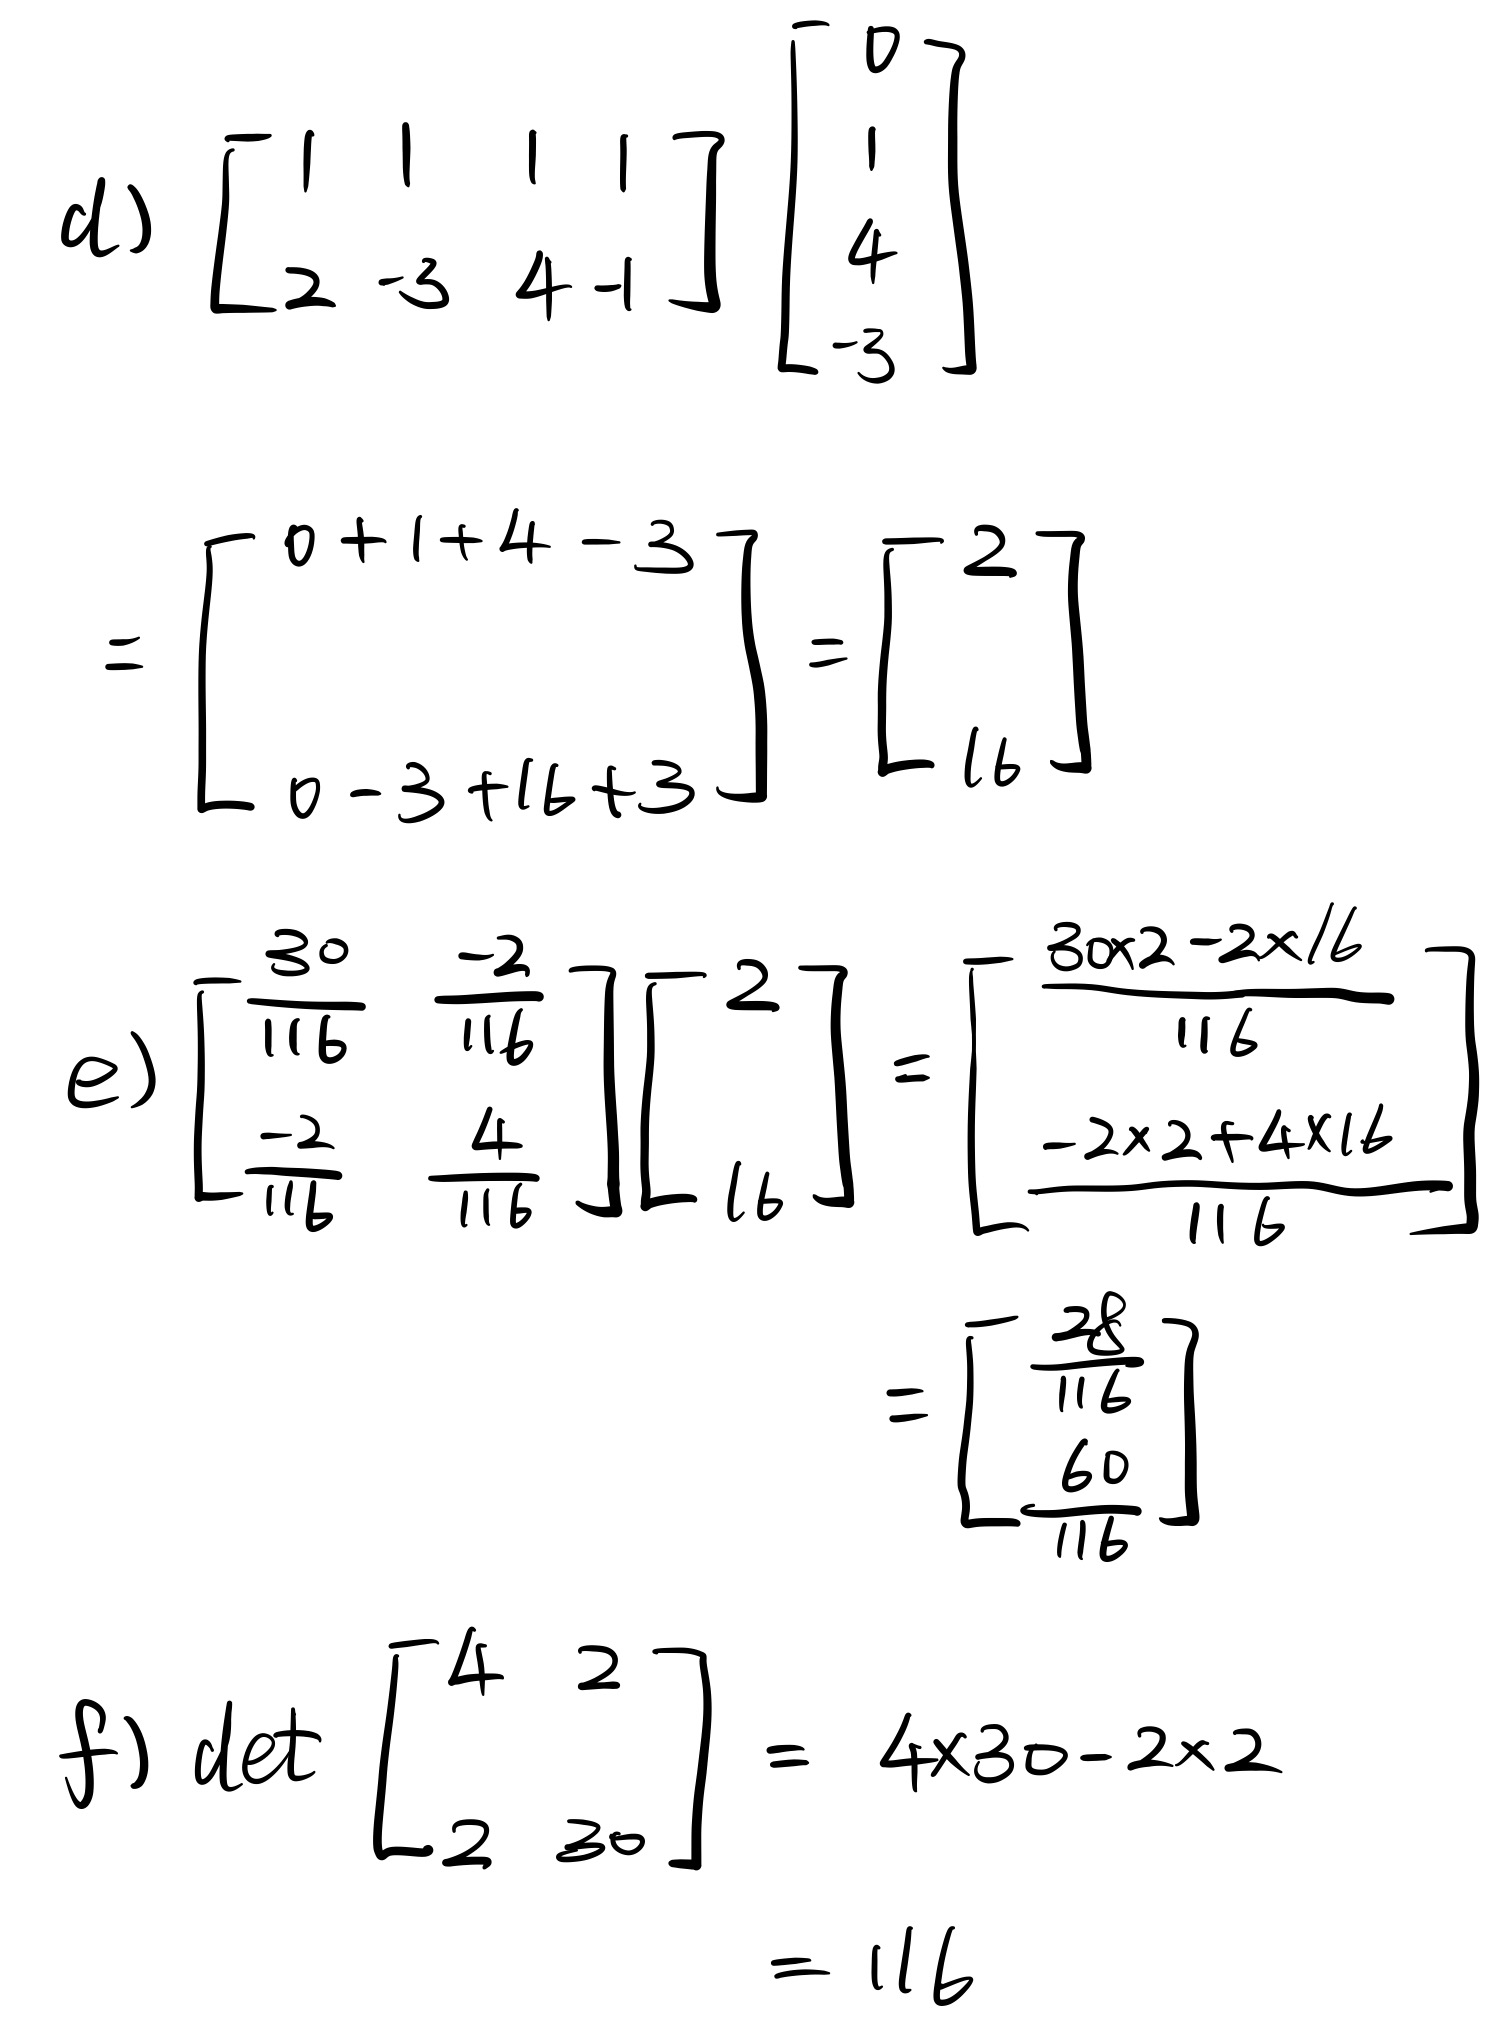
\includegraphics[width=0.7\textwidth]{figure2_Rplot.jpg}
	\end{figure}
\end{solution}

\newpage
%problem 2
\begin{problem}{2}
\textbf{[10 pts]}
In R, write a script to compute each of the parts in problem 1 to check your answers. Submit both the .r commands and the output. Then, create a dataset with $x = <2, -3, 4, -1>$ and $y = <0, 1, 4, -3>$ and run a regression analysis on the data with “lm”. Compare your value for $\beta$ in part e of the last problem, with the coefficients calculated by R's lm function.
\end{problem}
\begin{solution}
\href{run:./src/p2.r}{ (Problem 2 Source Code)}
\begin{lstlisting}
# output
> p1
     [,1] [,2] [,3] [,4]
[1,]    1    1    1    1
[2,]    2   -3    4   -1
> p2
     [,1] [,2]
[1,]    4    2
[2,]    2   30
> p3
            [,1]        [,2]
[1,]  0.25862069 -0.01724138
[2,] -0.01724138  0.03448276
> p4
     [,1]
[1,]    2
[2,]   16
> p5
          [,1]
[1,] 0.2413793
[2,] 0.5172414
> p6
[1] 116
> summary(fit)
Coefficients: (1 not defined because of singularities)
            Estimate Std. Error t value Pr(>|t|)
(Intercept)   0.2414     1.4931   0.162    0.886
Z1                NA         NA      NA       NA
Z2            0.5172     0.5452   0.949    0.443
\end{lstlisting}
Intercept of 0.2414 and slope of 0.5172 is exactly same as we derived at part (e).
\end{solution}

\newpage
%problem 3
\begin{problem}{3}
\textbf{[10 pts]}
Use the dataset “mtcars” which is built-in RStudio. You can see the structure of the data by the command “head(mtcars)”. Use the “mpg” column as your dependent variable Y, and do the following:
\begin{enumerate}
	\item Create a copy of the dataset called $A$ with only the columns $[cyl, disp, hp, wt, carb]$. Use the column selection mechanism we covered in class to select these columns from the dataset.
	\item Add a column of “ones” to $A$ called “count”.
	\item Use the “as.matrix” function to convert it to a matrix and assign it back to the variable $A$ (so you
are overwriting the data.frame here and converting it to a matrix)
	\item Compute the following multiple regression by manually computing the matrix operations:
	\newline
	$(A^TA)^{-1}A^TY$.
	\item Compute the regression with the RStudio “lm” command and compare with your results from d).
Note any differences.
\end{enumerate}
\end{problem}
\begin{solution}
\href{run:./src/p3.r}{ (Problem 3 Source Code)}
	\begin{lstlisting}
# output
> beta
              [,1]
cyl   -1.291898563
disp   0.011485584
hp    -0.020352893
wt    -3.846949031
carb  -0.006746893
count 40.815359236
> summary(fit)

Call:
lm(formula = Y ~ A)

Residuals:
    Min      1Q  Median      3Q     Max 
-4.0635 -1.4580 -0.4306  1.2927  5.8244 

Coefficients: (1 not defined because of singularities)
             Estimate Std. Error t value Pr(>|t|)    
(Intercept) 40.815359   3.025568  13.490    3e-13 ***
Acyl        -1.291899   0.679227  -1.902  0.06830 .  
Adisp        0.011486   0.015375   0.747  0.46175    
Ahp         -0.020353   0.020062  -1.015  0.31968    
Awt         -3.846949   1.192155  -3.227  0.00337 ** 
Acarb       -0.006747   0.574269  -0.012  0.99072    
Acount             NA         NA      NA       NA    
	\end{lstlisting}
All fitted slopes and intercept are same as we expected. 
\end{solution}

\newpage
%problem 4
\begin{problem}{4}
\textbf{[20 pts]}
Return to the housing dataset. In the last homework you conducted a regression with various methods of feature selection. In this problem you will turn to evaluating regression’s predictive power on this dataset, whether it is overfitting and investigate the performance of regularized regression. For this, I have provided you with the data divided into test and training sets.
\begin{enumerate}
	\item Rerun your full (all predictors) linear regression model of MEDV, using the training set and then calculate and report the $R^2$ and RMSE of the residuals. Then predict the y-values in the test set using this model. What is the RMSE for the test set? Is there evidence of overfitting here?
	\item Use cross-validated ridge regression on the training set and plot the relationship between the cross-validated error and log-lambda. Then use the model for predicting again the y’s in the test set using the “lambda.1se”. Report the $R^2$ for the training set (how do you get this?) and the RMSE for both the training and test set. How do these compare to the OLS regression model? Are they improving prediction? If so, how?
	\item Do the same as in b) for Lasso using “lambda.1se”. How do the results compare to Ridge and OLS regression? Also, for Lasso, evaluate how the number of variables changes with lambda. How many variables are selected at lambda.1se? Finally, how do the variables selected, and their betas computed compare with the model you got last week with stepwise regression?
	\item Revisit the cross-validated error graphs for both Ridge and Lasso, and evaluate how well regularization is working for this set? Is there a strong indication that cross-validated error can be reduced by regularization in this case? What do you think this mean for overfitting in the original model?
\end{enumerate}
\end{problem}
\begin{solution}
\href{run:./src/p4.r}{ (Problem 4 Source Code)}
\begin{enumerate}
	\item \mbox{}
	Housing training dataset has $R^w$ of 0.7571 and RMSE of 4.580769, housing test dataset has RMSE of 5.263608. The 15\% lager RMSE in test dataset indicate the overfitting.
	\begin{lstlisting}
# output
> summary(fit)
Coefficients:
              Estimate Std. Error t value Pr(>|t|)    
(Intercept)  3.965e+01  5.610e+00   7.069 7.94e-12 ***
CRIM        -1.299e-01  3.412e-02  -3.807 0.000165 ***
ZN           4.341e-02  1.570e-02   2.764 0.005994 ** 
INDUS        6.302e-03  6.958e-02   0.091 0.927884    
CHAS         3.594e+00  9.454e-01   3.802 0.000168 ***
NOX         -2.197e+01  4.377e+00  -5.021 8.05e-07 ***
RM           4.229e+00  4.898e-01   8.634  < 2e-16 ***
AGE         -1.268e-04  1.511e-02  -0.008 0.993307    
DIS         -1.529e+00  2.318e-01  -6.598 1.46e-10 ***
RAD          2.665e-01  7.341e-02   3.630 0.000324 ***
TAX         -1.134e-02  4.130e-03  -2.746 0.006338 ** 
PTRATIO     -9.828e-01  1.506e-01  -6.526 2.24e-10 ***
LSTAT       -4.665e-01  6.094e-02  -7.655 1.73e-13 ***
---
Residual standard error: 4.661 on 367 degrees of freedom
Multiple R-squared:  0.7571,	Adjusted R-squared:  0.7491 
F-statistic: 95.31 on 12 and 367 DF,  p-value: < 2.2e-16
> housingTrainDataRMSE
[1] 4.580769
> housingTestDataRMSE                                              
[1] 5.263608
	\end{lstlisting}
	\item \mbox{}
	Ridge regression provide a better model. Compare to previous linear model RMSE of 4.580769, ridge regression has RMSE of 5.647947 which lead to the whole model non-overfitting, and the different between training and testing data from 15\% to 6.8\%.
	\begin{figure}[h]
		\centering
		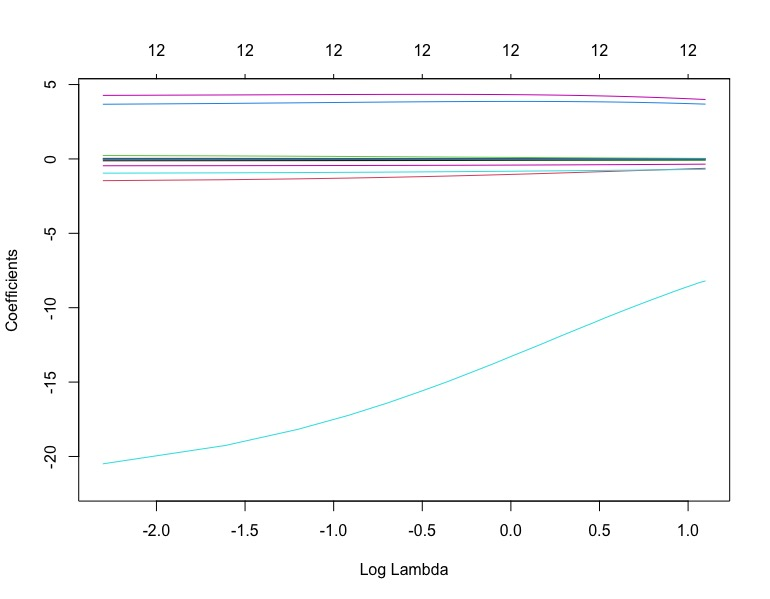
\includegraphics[width=0.8\textwidth]{figure3_Rplot.jpeg}
		\caption{Relationship Between the Cross-Validated Error and Log-lambda}
	\end{figure}	
	\begin{lstlisting}
# output
> housingTrainRidgeFit

Call:  glmnet(x = housingTrainOther, y = housingTrainMEDV, alpha = 0,      lambda = seq(0, 3, 0.1)) 

   Df  %Dev Lambda
1  12 72.42    3.0
2  12 72.54    2.9
3  12 72.66    2.8
4  12 72.78    2.7
5  12 72.90    2.6
6  12 73.01    2.5
7  12 73.13    2.4
8  12 73.25    2.3
9  12 73.37    2.2
10 12 73.49    2.1
11 12 73.61    2.0
12 12 73.73    1.9
13 12 73.84    1.8
14 12 73.96    1.7
15 12 74.08    1.6
16 12 74.20    1.5
17 12 74.32    1.4
18 12 74.43    1.3
19 12 74.55    1.2
20 12 74.67    1.1
21 12 74.78    1.0
22 12 74.90    0.9
23 12 75.01    0.8
24 12 75.13    0.7
25 12 75.23    0.6
26 12 75.34    0.5
27 12 75.44    0.4
28 12 75.54    0.3
29 12 75.62    0.2
30 12 75.68    0.1
31 12 75.71    0.0
> rmseRidge
[1] 5.647947
	\end{lstlisting}
	\item \mbox{}
	Lasso regression provide a better model. Totally we have 8 variables selected, lasso regression has RMSE of 5.434684 which significantly decrease the different between training and testing data from 15\% to 3.1\%. RMSE is dramatically increase when there are fewer than 8 variables or even less include.
	\begin{figure}[h]
		\centering
		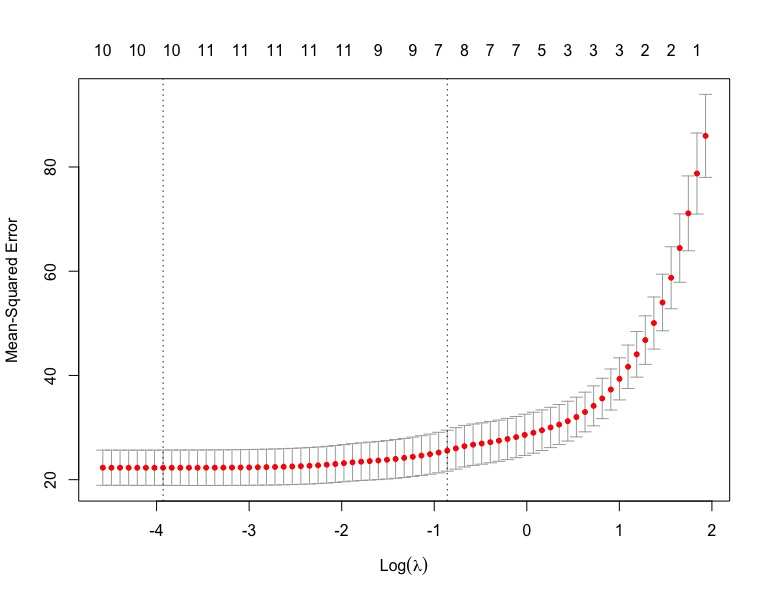
\includegraphics[width=0.8\textwidth]{figure4_Rplot.jpeg}
		\caption{Relationship Between the Cross-Validated Error and Log-lambda}
	\end{figure}	
	\newpage
	\begin{lstlisting}
# output
> rmseLasso 
[1] 5.434684
> coef(housingTrainLassoFit2, s="lambda.1se")
13 x 1 sparse Matrix of class "dgCMatrix"
                       s1
(Intercept)  1.831834e+01
CRIM        -4.637730e-02
ZN           .           
INDUS        .           
CHAS         2.996345e+00
NOX         -6.676971e+00
RM           4.652014e+00
AGE          .           
DIS         -2.261454e-01
RAD          .           
TAX         -4.392951e-05
PTRATIO     -8.040975e-01
LSTAT       -4.531617e-01	
	\end{lstlisting}
	\item \mbox{}
	We could apply cross validation multiple times, if all of our estimates give similar outputs, we can be more certain of the model’s accuracy. Meanwhile, if our estimates give different outputs, that tells us the model does not perform consistently and suggests a problem with it.
\end{enumerate}
\end{solution}

\newpage
%problem 5
\begin{problem}{5}
\textbf{[20 pts]}
The data in the files insurTest.csv and insurTrain.csv are collected from 47 zip-code areas in the Illinois area. There are 8 columns in the data file but not all are relevant here. The response variable of interest is the number of new home insurance policies (NEWPOL) (minus canceled policies) per 100 housing units. The predictor variables are the percent minority population living in the area (PCTMINOR), the number of fires per 1000 housing units (FIRES), the number of thefts per 1000 in population (THEFTS), the percent of housing units built before 1940 (PCTOLD), and the median income (INCOME).
\begin{enumerate}
	\item Run a multiple regression of NEWPOL on the variables: PCT-MINOR FIRES THEFTS PCTOLD INCOME NEWPOL.
	\item Use the model from a) to predict the test set. What is the RMSE here? Is there evidence of overfitting?
	\item Run a ridge regression on the training set, produce the lambda plot, and report the RMSE for both the training and test sets using lambda.1se. From the lambda plot, how well is regularization working here? Look at the shape of the plot for a significant dip before it rises.
	\item Run a lasso regression on the training set, produce the lambda plot, and report the RMSE for both the training and test sets using lambda.1se. Compare them with those you got in c). Are they closer together, more stable, or have they worsened overall?
	\item Plot the residuals vs the fitted (predicted values), you can do this with plot(fitted, residuals) since you’ve calculated both in order to get the RMSE (remember, residuals are the difference between actual and predicted). Does the lasso add any significant bias into the model? Note that it may or may not show up as a slope difference. It could also appear as a mean residual different from 0 as well.
	\item Use Elastic Net regression and determine if there is an alpha between 0 and 1 that will give a better result with this test and training set. Try alphas of .25, .5 and .75. Does it appear that there might be an alpha that does better than either ridge or lasso?
	\item Is there a practical reason to try and mix lasso and ridge here? Explain your answer.
\end{enumerate}
\end{problem}
\begin{solution}
\href{run:./src/p5.r}{ (Problem 5 Source Code)}
\begin{enumerate}
	\item \mbox{}
	\begin{lstlisting}
# output
> summary(fit)
Coefficients:
              Estimate Std. Error t value Pr(>|t|)    
(Intercept) 13.1561459  3.1181250   4.219 0.000577 ***
pctmin      -0.0506103  0.0203648  -2.485 0.023654 *  
fires       -0.1148724  0.0532530  -2.157 0.045603 *  
thefts      -0.0983249  0.0312860  -3.143 0.005934 ** 
pctold      -0.0628540  0.0215552  -2.916 0.009631 ** 
income       0.0003252  0.0002103   1.546 0.140407    
---
Residual standard error: 1.303 on 17 degrees of freedom
Multiple R-squared:  0.9272,	Adjusted R-squared:  0.9058 
F-statistic: 43.32 on 5 and 17 DF,  p-value: 4.387e-09
> insurTrainDataRMSE
[1] 1.120282
	\end{lstlisting}
	Overall model fit has p-value of $4.387\times 10^{-9}$, $R^2$ of 0.9272 which indicates a very well fit model. Notice also that 4 out of 5 independent variables have significant coefficients at an alpha of .05. PCTMIN, FIRES, THEFTS, and PCTOLD all show significantly different coefficients than 0 suggesting a one unit change in these variables predicts a reliable change in NEWPOL. Lastly, the linear regression model has RMSE of 1.120282.
	\item \mbox{}
	Predict model RMSE is 4.260169, which is much larger than training data RMSE of 1.120282, this is good evidence that overfitting is a potential issue in our model.
	\item \mbox{}
	RMSE for ridge regression is 15.37505.
	\item \mbox{}
	RMSE for lasso regression is 15.37505, there is no change compare to ridge regression
	\item \mbox{}
	\begin{figure}[h]
		\centering
		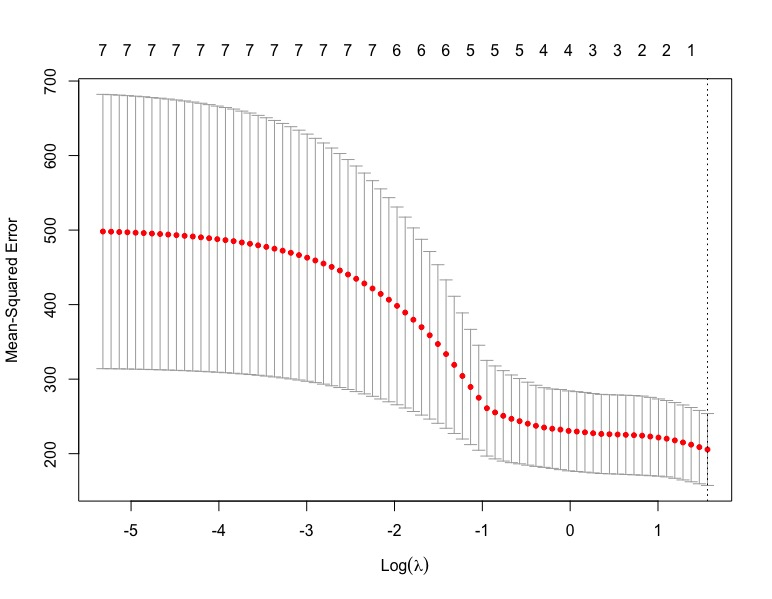
\includegraphics[width=0.8\textwidth]{figure5_Rplot.jpeg}
		\caption{Relationship Between the Cross-Validated Error and Log-lambda}
	\end{figure}	
	\item \mbox{}
	RMSE for elastic net regression is 15.37505 for all 3 different alpha (0.25, 0.5 and 0.75).
	\item \mbox{}
	From result, all three different regression provide same RMSE value, there might be some technique problem in my code or there is no reason to try mix lasso and ridge.
\end{enumerate}
\end{solution}

\newpage
%problem 6
\begin{problem}{6}
\textbf{[20 pts]}
Read and review the posted paper “Adding bias to reduce variance in psychological results.” Most of the mathematics here will be similar to what we’ve gone over in class but pay particular attention to Section 3: Examples. Answer the following questions, in detail. You should be able to write a detailed paragraph about each of at least three or four complete sentences with
\begin{enumerate}
	\item What is the size of the dataset relative to the number of independent variables?
	\item Is there evidence of overfitting in their dataset?
	\item How are regularized regression techniques being used in their examples?
	\item How do the results of regularized regression differ from the OLS model?
	\item How do they evaluate the performance of each of the regularized regression techniques?
	\item Are there any issues that you can identify with the way that they are evaluating this
performance?
\end{enumerate}
\end{problem}
\begin{solution}
\begin{enumerate}
	\item  According to the abstract, the goal is to predict student math exam performance using 30 potential predictors. The observed number appears to be n = 395 Portuguese students. This results in a 395 x 30 dataset with 30 potential predictor values. Binary, categorical, and integer values are used to measure everything from student sex to commute time to school and weekend alcohol consumption. Due to the multiple levels, the categorical variables were recoded into dummy variables, yielding a total of 39 predictor variables.
	\item There appears to be some evidence of overfitting, as evidenced by their OLS model's high average MSE of 9.3. The moderate size of the data in relation to the large number of terms also suggests that there may be overfitting issues, as the coefficients may represent noise rather than the true relationships of the data. Each of these terms in the model forces the regression to try to estimate each of these parameters, which results in the regression simply tracing noise.
	\item Regularized regression, or penalized regression, as it is referred to in the paper, is being investigated to address the issues associated with using maximum likelihood estimates to find coefficients in moderate size data. They want to investigate various methods of introducing bias into estimators in the hopes of reducing variance. They hope that by using regularized regression techniques, they will be able to provide better solutions that are more representative of the population as a whole rather than just the sample.
	\item When the models are compared, the OLS consistently has higher coefficients than the Ridge model, but both keep all coefficients at non-zero values. The Lasso model assisted in both coefficient size reduction and variable selection, which the OLS does not. The Elastic net model outperformed the OLS while avoiding some of the pitfalls that Lasso overlooks, such as high multicollinearity among predictors. The RMSE values appear to be slightly lower in the majority of the models tested. All three models used introduced bias in the hopes of lowering the coefficients and making the models more representative or reliable of actual relationships.
	\item To assess the performance of the various models, an auxiliary simulation is run to compare MSPE across test sets for different models. They then compared the mean square prediction errors of the various models to determine how much additional error was produced by the test sets. They then investigated the variability of MSPE values due to random sampling by running 100 different random data splits (test and training sets) for each of the ten methods. They then averaged and compared the MSPE values of each method. They discovered that Lasso and Elastic net worked best with Ridge following.
	\item One of the mistakes was not comparing the MSPE of the training set to that of the test set. This would have provided a more relative perspective on how the models handled differences in data set error relative to what the model produced. They could also have used more than one dataset because it is likely that there were extremely similar datasets out of 100 iterations of splitting the dataset of only 359 observations, which breaks down what they were attempting to address.
\end{enumerate}
\end{solution}

\end{document}